\documentclass[conference]{IEEEtran}

\IEEEoverridecommandlockouts

\usepackage{amsmath,amssymb}
\usepackage{graphicx}
\usepackage{booktabs}
\usepackage{multirow}
\usepackage{array}
\usepackage{xcolor}
\usepackage{cite}
\usepackage{url}
\usepackage{needspace}
\usepackage{balance}

\renewcommand{\topfraction}{0.95}
\renewcommand{\bottomfraction}{0.90}
\renewcommand{\textfraction}{0.05}
\renewcommand{\floatpagefraction}{0.85}
\renewcommand{\dbltopfraction}{0.95}
\renewcommand{\dblfloatpagefraction}{0.85}
\setlength{\textfloatsep}{8pt plus 2pt minus 2pt}
\setlength{\floatsep}{7pt plus 2pt minus 2pt}
\setlength{\dbltextfloatsep}{9pt plus 2pt minus 2pt}
\setlength{\dblfloatsep}{7pt plus 2pt minus 2pt}

\graphicspath{{../figures/synergy_manuscript/}}

\title{What Does Random Splitting Evaluate in Drug Synergy Benchmarks?\\A Repeated-Entity Audit}

\author{
\IEEEauthorblockN{
Yuxin Wen\textsuperscript{\(\dagger\)},
Yi Tian\textsuperscript{\(\dagger\)},
Nguyen Quoc Khanh Le\textsuperscript{*,\(\ddagger\),\P,\S},
and Matthew Chin Heng Chua\textsuperscript{*,\(\dagger\)}
}
\IEEEauthorblockA{
\textsuperscript{\(\dagger\)}Department of Biomedical Informatics, Yong Loo Lin School of Medicine,\\
National University of Singapore, Singapore 119615, Singapore\\
\textsuperscript{\(\ddagger\)}In-Service Master Program in Artificial Intelligence in Medicine, College of Medicine,\\
Taipei Medical University, Taipei 110, Taiwan\\
\textsuperscript{\P}AIBioMed Lab, Taipei Medical University, Taipei 110, Taiwan\\
\textsuperscript{\S}Translational Imaging Research Center, Taipei Medical University Hospital, Taipei 110, Taiwan\\
\textsuperscript{*}Corresponding authors: khanhlee@tmu.edu.tw; matthewchua@nus.edu.sg
}
}

\begin{document}

\maketitle

\begin{abstract}
Large drug-combination tables contain many rows but comparatively few recurring drugs, unordered pairs, and cell lines. We study how this repeated-entity structure shapes random-split evaluation. Our audit uses 287,268 DrugComb ZIP examples, train-only global and entity-prior controls, a symmetric identity ridge, Morgan-fingerprint and hash-feature baselines, compact neural baselines, and six evaluation protocols. The processed benchmark contains 129 drugs, 5,427 unordered pairs, and 59 cell lines; under random splitting, all drugs and cells and more than 99.99\% of test pairs are already represented in training. Across three full-table random splits, identity ridge reaches RMSE $4.323\pm0.016$, compared with $4.708\pm0.020$ for ECFP ridge and $4.920\pm0.026$ for hash ridge; additive prior reaches $4.329\pm0.017$. Removing exact pair reuse contracts the identity--hash gap from 0.597 to 0.080 RMSE. On the common 30k suite, identity ridge, additive prior, and hash ridge become comparable when every test pair contains at least one drug unseen in training, whereas ECFP ridge and the compact MLPs are weaker. A separately processed NCI-ALMANAC table also exhibits strong random-split pair, additive, and identity controls. Conditional coupling and prototype-residual experiments further characterize prediction--prior dependence and feature-removal sensitivity. Together, the results show that random row splitting substantially rewards repeated-entity interpolation and that row count alone overstates the diversity of independent evaluation contexts.
\end{abstract}

\begin{IEEEkeywords}
drug synergy prediction, benchmark reliability, repeated entities, data-centric AI, cold-start evaluation, DrugComb
\end{IEEEkeywords}

\section{Introduction}

Drug combinations can improve efficacy, reduce resistance, and target complementary cancer pathways. Public resources such as DrugComb and NCI-ALMANAC have consequently enabled predictive modeling of synergy at substantial scale \cite{drugcomb2019,drugcombdb2020,nci2019almanac}. Models range from descriptor-based neural networks to dual-view, graph, transformer, and multitask architectures \cite{deepsynergy2018,matchmaker2022,deepdds2022,transynergy2021,marsy2023}. Their evaluation, however, is inseparable from how drug-pair--cell-line triples are partitioned.

Evaluation diversity in this setting is governed by the repeated-entity graph together with the row count. After duplicate aggregation, the DrugComb table used here has 287,268 rows but only 129 drugs, 5,427 unordered pairs, and 59 cell lines. A random row split places all drugs and cells and more than 99.99\% of test pairs in both training and test sets. Models can then exploit train-estimated entity tendencies, whether through explicit identifiers or features correlated with them. Random-split accuracy consequently combines transferable interaction learning with interpolation over familiar entities.

This issue connects drug synergy prediction to broader work on shortcut learning \cite{geirhos2020shortcut,brown2023shortcut}, cold-start evaluation \cite{dewulf2021cold}, and leakage-reduced biochemical splitting \cite{datasail2025}. Recent synergy evaluation studies likewise distinguish leave-triple, leave-pair, unseen-drug, and unseen-cell settings \cite{marsy2023,synverse2025}. We quantify prediction--prior association as \emph{coupling} and examine how it changes across split regimes.

This paper asks three ordered questions. First, how severe is train--test entity repetition? Second, how much random-split performance can be explained by models that use only training-set identities or entity response tendencies? Third, how does the conclusion change when pair, drug, or cell reuse is removed? Figure~\ref{fig:overview} summarizes this audit. Conditional coupling and Cluster-Prototype-Based (CPB) residualization are retained only as supporting diagnostics for interpreting the three primary questions.

\begin{figure*}[!t]
    \centering
    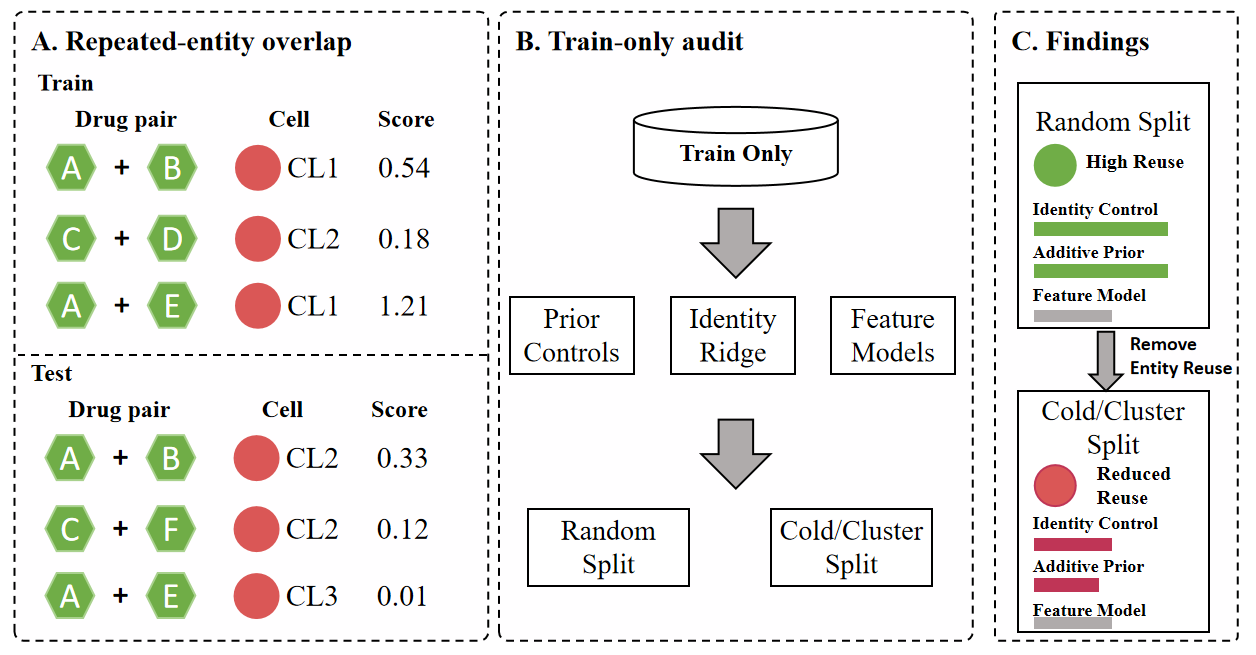
\includegraphics[width=0.96\textwidth]{fig1_overview_simplified.png}
    \caption{Overview of the repeated-entity audit. (a) Random row splitting reuses drugs, unordered pairs, and cell lines across training and test data. (b) Train-only prior and identity controls are compared with feature models under random and cold/cluster splits. (c) Their high-reuse advantage contracts as reuse is reduced. Bars are schematic.}
    \label{fig:overview}
\end{figure*}

The study makes three primary contributions:
\begin{itemize}
    \item We quantify the benchmark's repeated-entity structure using full-table frequency and train--test overlap audits, revealing the effective combination contexts represented by 287,268 rows.
    \item We show that train-only identity and entity-prior controls match or outperform controlled feature and neural models under random splitting, establishing the predictive signal available from entity identities and response tendencies.
    \item We compare random evaluation with five split stresses and show that the random-split advantage contracts, disappears, or changes interpretation as exact-pair, drug, or cell reuse is removed; strong entity-only random-split predictability is also observed on NCI-ALMANAC.
\end{itemize}

Coupling, synthetic, prototype-residual, label-robustness, uncertainty, and runtime analyses connect the primary finding to diagnostic behavior, statistical stability, and computational cost. The resulting workflow provides a lightweight benchmark audit that can accompany evaluations of domain-specific architectures.

\section{Related Work}

\subsection{Drug synergy prediction}

DeepSynergy combined chemical descriptors and genomic features in a feed-forward network \cite{deepsynergy2018}. MatchMaker learned two drug--cell views \cite{matchmaker2022}; DeepDDS used molecular graphs and attention \cite{deepdds2022}; and TranSynergy integrated mechanism-informed features with self-attention \cite{transynergy2021}. MARSY used pair and triple encoders with auxiliary single-drug response tasks \cite{marsy2023}. GraphSynergy, PRODeepSyn, and MMSyn further integrate biological networks, protein interactions, or multimodal molecular evidence \cite{graphsynergy2021,prodeepsyn2022,mmsyn2024}. ChemicalX provides reusable implementations for drug-pair scoring architectures \cite{chemicalx2022}. Our controlled neural baselines instantiate descriptor and dual-view design patterns over the common features available in the TDC task table.

Benchmark design has become a first-order concern. MARSY reports leave-triple and leave-pair evaluation \cite{marsy2023}. SynVerse systematically studies unseen triples, pairs, drugs, and cells and reports that one-hot baselines can remain difficult to beat \cite{synverse2025}. Cold-start work in drug--drug interactions distinguishes one-new-drug from two-new-drug tasks \cite{dewulf2021cold}, while DataSAIL formalizes similarity-aware splitting for biochemical data \cite{datasail2025}. The AstraZeneca--Sanger challenge winner also used cross-drug and cross-cell information under a common community evaluation \cite{networkprop2018}. Our audit adds a full-table entity-frequency analysis, continuous train-only response priors, grouped uncertainty, five complementary reuse-removal stresses, and a separately processed NCI-ALMANAC check.

\subsection{Synergy data and reliability}

DrugComb integrates heterogeneous screening sources and multiple synergy definitions \cite{drugcomb2019}; DrugCombDB similarly emphasizes curation across high-throughput studies and literature \cite{drugcombdb2020}. Different non-interaction models can produce materially different labels, motivating label robustness checks \cite{amzallag2019,musyc2021}. The NCI-DREAM challenge also demonstrated the importance of controlled community evaluation \cite{bansal2014}. Therapeutics Data Commons standardizes access to therapeutic tasks \cite{tdc2021}. We record the study, dose-grid, assay, and batch fields available in the distributed table to determine which source-aware splits can be constructed.

Prior-bias diagnostics have also been developed for drug--target interaction prediction, including intervention-based controls for target-level response tendencies \cite{lin2025tapb}. We extend this evaluation perspective to continuous drug-synergy scores and repeated drug, pair, and cell entities.

\section{Audit Framework}

\subsection{Train-only prior controls}

Each example is an unordered drug pair in a cell-line context,
\begin{equation}
x_i=(d_{i1},d_{i2},c_i), \qquad y_i\in\mathbb{R}.
\end{equation}
All priors are estimated on the training split. For entity group $g$, empirical-Bayes shrinkage gives
\begin{equation}
\widetilde{\mu}_g=\mu_0+\frac{n_g}{n_g+\tau}(\bar y_g-\mu_0),\qquad \tau=10.
\end{equation}
Drug, unordered-pair, and cell tendencies are denoted $p_D$, $p_P$, and $p_C$. Unseen entities fall back to the global mean for marginal priors and zero for residual effects.

The additive prior is explicit:
\begin{equation}
\hat y_{\mathrm{add}}=\mu_0+a_{d_1}+a_{d_2}+b_{\{d_1,d_2\}}+c_c.
\end{equation}
It is fitted in one pass using the fixed order drug $\rightarrow$ pair $\rightarrow$ cell. Drug effects use half of the centered row residual for each constituent drug; pair effects are fitted to the remaining residual; and cell effects are fitted last. Each stage uses the same shrinkage rule. This construction provides a reproducible train-only control for lower-order entity tendencies.

\subsection{Supporting coupling diagnostics}

For available prior components $\mathcal A_s$ in split $s$, ordinary PCS is
\begin{equation}
\mathrm{PCS}_s=\frac{1}{|\mathcal A_s|}\sum_{r\in\mathcal A_s}|\mathrm{corr}(\hat y,p_r)|.
\end{equation}
We report $|\mathcal A_s|$ and also a fixed-denominator form,
\begin{equation}
\mathrm{PCS}^{(3)}_s=\frac{1}{3}\sum_{r\in\mathcal A_s}
\left|\mathrm{corr}(\hat y,p_r)\right|.
\end{equation}
A prior with zero variance is marked unavailable and contributes zero to the fixed-denominator score. In cold-both-drugs, the cell prior is the only varying component.

Because $p_r$ can be genuinely correlated with $y$, we add conditional PCS:
\begin{equation}
\mathrm{cPCS}_s=\frac{1}{|\mathcal A'_s|}\sum_{r\in\mathcal A'_s}
\left|\mathrm{corr}\{e(\hat y\mid y),e(p_r\mid y)\}\right|,
\end{equation}
where $e(z\mid y)$ is the residual from a linear regression of $z$ on $y$, and $\mathcal A'_s\subseteq\{D,P,C\}$ contains prior components with non-zero residual variance after conditioning on $y$. This partial correlation measures prediction--prior association after removing their shared linear relationship with the observed label. For comparisons across splits, we use
\begin{equation}
\mathrm{cPCS}^{(3)}_s=\frac{1}{3}\sum_{r\in\mathcal A'_s}
\left|\mathrm{corr}\{e(\hat y\mid y),e(p_r\mid y)\}\right|.
\end{equation}
Prior components with zero residual variance are unavailable and contribute zero to $\mathrm{cPCS}^{(3)}_s$.

We also report incremental prior explanation,
\begin{equation}
\Delta R^2_P=R^2(\hat y\sim y,p_D,p_P,p_C)-R^2(\hat y\sim y).
\end{equation}
A 64-replicate moment-matched heuristic null provides a secondary check. Each null prediction combines standardized $y$ with Gaussian noise orthogonal to $y$, then matches the observed prediction mean, variance, Pearson correlation with $y$, and RMSE. We summarize the difference between observed PCS and mean null PCS as PCS excess.

All coupling quantities are interpreted alongside RMSE and Pearson correlation.

\subsection{Supporting synthetic sanity check}

Across 20 synthetic seeds, we compare label-only prediction, direct residual-prior use, and nonlinear label--prior association while fixing RMSE to 1.0. Adjusted diagnostics should be near zero in the first and third cases and positive only under direct prior use.

\subsection{Supporting prototype-residual stress test}

CPB measures prediction sensitivity to prototype-level feature removal. Character-level SMILES hashes and cell identifiers are projected to pair and cell embeddings $u$ and $v$ of dimension 16. Training-only MiniBatchKMeans centroids define
\begin{align}
a(u)&=\arg\min_k\|u-\pi_k\|_2^2, &
r_P^{(\lambda)}&=u-\lambda\pi_{a(u)},\\
b(v)&=\arg\min_l\|v-\gamma_l\|_2^2, &
r_C^{(\lambda)}&=v-\lambda\gamma_{b(v)}.
\end{align}
\begin{equation}
\phi_{\mathrm{res}}^{(\lambda)}
=[r_P^{(\lambda)},r_C^{(\lambda)},
r_P^{(\lambda)}\odot r_C^{(\lambda)}].
\label{eq:residual-map}
\end{equation}
We sweep $\lambda\in\{0,0.25,0.50,0.75,1.00\}$ and $(K_P,K_C)\in\{(8,4),(16,8),(32,16)\}$. Learned centroids use MiniBatchKMeans with $n_{\rm init}=10$ on distinct training entities. The shuffled-assignment control assigns each entity to a learned centroid by a deterministic seed-specific hash; the random-cluster control randomly partitions training embeddings and uses the resulting group means. Both controls are rescaled to match the learned setting's mean squared assigned-centroid norm before residualization. Ridge regression is then fitted on each residual map. Results use seeds 0, 42, and 123, and each plotted point is the mean of the corresponding setting across seeds.

\section{Experimental Setup}

\subsection{Data audit and preprocessing}

The primary table is the DrugComb task distributed through TDC \cite{tdc2021}. We canonicalize unordered pairs, remove missing identifiers, SMILES, cells, or labels, and aggregate duplicate pair--cell rows by median score before splitting. Each retained drug identifier maps to one SMILES string after preprocessing. ZIP is primary; Bliss, Loewe, and HSA support label checks. The resulting ZIP table has 287,268 rows. Pair--cell multiplicity is exactly one after aggregation.

The distributed task table contains drug identifiers, SMILES, cell identifiers/names, CSS, and four synergy labels. Study, source, assay, dose-grid, publication, and batch columns are absent, so the available split audit focuses on drug, pair, cell, and representation-defined partitions. NCI-ALMANAC is processed separately from CellMiner 2.15 into 306,365 drug-pair--cell records containing 104 drugs, 5,233 unordered pairs, and 59 cells; duplicate triples are median aggregated. Under each of its three random splits, every test drug, pair, and cell is represented in training. Its broader score range is analyzed on its native scale.

\begin{table}[!t]
\centering
\caption{Full DrugComb entity-frequency audit after preprocessing. Drug occurrence counts both drug positions in each combination row.}
\label{tab:frequency}
\begin{tabular}{lrrrr}
\toprule
Entity & Unique & Median & Max & Gini \\
\midrule
Drug occurrence & 129 & 5,667 & 5,937 & 0.224 \\
Unordered pair & 5,427 & 58 & 59 & 0.094 \\
Cell line & 59 & 4,849 & 5,384 & 0.025 \\
Pair--cell row & 287,268 & 1 & 1 & 0.000 \\
\bottomrule
\end{tabular}
\end{table}

The full occurrence distributions in Fig.~\ref{fig:support}a reveal the structure behind the row count. Unordered pairs are especially concentrated near 58--59 observations because most are measured across nearly the complete cell-line panel, while drugs and cells recur across thousands of rows. Thus the 287,268 rows form a dense repeated-entity graph with 5,427 distinct pair contexts.

\subsection{Sampling and splits}

The full table is used for the data audit, scale experiment, and three-seed critical-model comparison on random, cold-pair, and cold-both-drugs splits. The broader six-protocol comparison, including ECFP ridge and both MLP proxies, uses a common 30k subset; CPB Pareto controls use a common 40k subset. Subsets are deterministic, nested, and stratified by ZIP decile. This keeps the neural and dense ablations resource-bounded while making every model within an experiment see identical rows. Scale sensitivity uses nested 25k, 50k, 100k, and full-table samples. The Bliss, Loewe, and HSA checks use the full table with seed 42 and report the identity-control RMSE change from random to cold splits, providing a split-level robustness comparison across four label definitions.

Random splits allocate 80/10/10\% of rows. Cold-pair partitions unordered pairs 80/10/10, and cold-cell similarly partitions cell identifiers. The \emph{cold-at-least-one-drug} protocol partitions drugs 80/10/10 and assigns a row to test if either drug belongs to the test set, otherwise to validation if either drug belongs to the validation set, and to training only when both drugs belong to the training set. Hence every row is assigned and every test pair contains at least one held-out drug. Cold-both-drugs partitions drugs 70/15/15, retains only train--train, validation--validation, and test--test pairs, and discards cross-group pairs. The representation-specific cluster stress fits 1,024 character 2--5-gram SMILES hashes, at most 24 SVD dimensions, and ten clusters to all unique drugs without using response labels; row assignment then follows the same test-first, validation-second priority as cold-at-least-one-drug. Across seeds, the mean nearest-training-drug hash cosine of held-out drugs is 0.625--0.667 (maximum 0.779--0.815). Seeds are 0, 42, and 123.

Seen ratios quantify the remaining reuse channel. Drug seen ratio is the fraction of the two drug slots across test rows whose drug identifier occurs in training. Pair and cell seen ratios are the fractions of test rows whose unordered pair or cell identifier, respectively, occurs in training.

\begin{table*}[!t]
\centering
\caption{Full-table cold-drug split sizes. One-new and both-new are test-row proportions. Distinct drugs counts all drugs appearing in the test partition, including both seen and held-out drugs. Cold-both-drugs discards cross-group pairs outside train--train, validation--validation, and test--test groups.}
\label{tab:split-sizes}
\begin{tabular}{llrrrrrrrr}
\toprule
Split & Seed & Train & Validation & Test & Discarded & Distinct drugs & Test pairs & One-new & Both-new \\
\midrule
\multirow{3}{*}{Cold-$\geq$1-drug} & 0   & 186,982 & 44,444 & 55,842 & 0       & 123 & 1,071 & 0.856 & 0.144 \\
 & 42  & 175,307 & 42,761 & 69,200 & 0       & 128 & 1,249 & 0.840 & 0.160 \\
 & 123 & 179,347 & 48,174 & 59,747 & 0       & 121 & 1,058 & 0.840 & 0.160 \\
\midrule
\multirow{3}{*}{Cold-both-drugs} & 0   & 136,341 & 7,661 & 5,449 & 137,817 & 20 & 111 & 0.000 & 1.000 \\
 & 42  & 121,975 & 7,876 & 8,624 & 148,793 & 19 & 154 & 0.000 & 1.000 \\
 & 123 & 129,085 & 6,909 & 7,938 & 143,336 & 18 & 138 & 0.000 & 1.000 \\
\bottomrule
\end{tabular}
\end{table*}

\subsection{Models, tuning, and compute}

Identity ridge uses one shared drug encoder and sums the two drug one-hot vectors, then concatenates unordered-pair and cell identities. This removes arbitrary canonical-slot coefficients. Hash ridge maps each SMILES to a 512-dimensional character 2--5-gram hashing vector. For drug vectors $h_1,h_2$, its symmetric pair block is $[h_1+h_2,|h_1-h_2|,h_1\odot h_2]$. Fixed Gaussian matrices with entries drawn from $\mathcal N(0,1/\sqrt{d_{\rm in}})$ project the pair block and training-fitted cell one-hot vector to 16 dimensions; their elementwise product supplies the interaction block. Projection seeds follow the split seeds. ECFP ridge uses radius-2, 2,048-bit Morgan fingerprints \cite{rogers2010ecfp} and the same sum, absolute-difference, and product pair operators, concatenated with a training-fitted cell one-hot vector. All ridge models use $\alpha=10$ and LSQR without split-specific tuning.

The descriptor MLP uses symmetric drug sum, absolute difference, product, cell, and pair--cell interactions. The dual-view MLP builds separate drug--cell views and combines their sum, absolute difference, and product, following the dual-view design pattern of MatchMaker with the available inputs. Inputs are standardized using training statistics. Both minimize squared error with ReLU hidden units, scikit-learn's seeded Glorot initialization, and Adam. They choose between $(128,64),\alpha=10^{-3}$ and $(128,64,32),\alpha=10^{-4}$ by outer-fold validation RMSE; each candidate uses a seeded internal 10\% training holdout for early stopping. Adam uses batch size 256, learning rate $10^{-3}$, at most 120 epochs, and stopping after ten non-improving epochs. Candidate and split random states are derived from seeds 0, 42, and 123. Experiments use an Intel Core i7-11800H CPU with 15.8 GB RAM, Python 3.11.15, RDKit 2026.3.4, and scikit-learn 1.9.0 \cite{sklearn2011}. OMP, MKL, OpenBLAS, and NumExpr are restricted to one thread. Reported runtimes include feature construction, fitting, and test inference.

\begin{table*}[!t]
\centering
\caption{Reproducible model and tuning configuration. All transformations are fitted on the training fold; the two MLP candidates receive the same validation-selection budget.}
\label{tab:config}
\begin{tabular}{p{0.16\textwidth}p{0.35\textwidth}p{0.40\textwidth}}
\toprule
Model & Representation & Estimator and selection \\
\midrule
Identity ridge & Sum of two shared drug one-hots, unordered pair, and cell; unknown categories ignored & Ridge, LSQR, $\alpha=10$; fixed for every split \\
Additive prior & Shrunk drug, pair, and cell residual effects; fixed drug $\rightarrow$ pair $\rightarrow$ cell order & One pass, $\tau=10$; no validation tuning \\
Hash ridge & 512 SMILES 2--5-gram hashes; symmetric pair blocks; 16-D Gaussian pair/cell projections and interaction & Ridge, LSQR, $\alpha=10$; projection follows split seed \\
ECFP ridge & Radius-2, 2,048-bit Morgan fingerprints; symmetric sum, absolute-difference, and product blocks; cell one-hot & Ridge, LSQR, $\alpha=10$; fixed for every split \\
Descriptor MLP & Standardized symmetric pair and pair--cell blocks & Adam; batch 256; LR $10^{-3}$; 120 epochs; choose $(128,64)/10^{-3}$ or $(128,64,32)/10^{-4}$ by validation RMSE \\
Dual-view MLP & Two standardized drug--cell views combined by sum, absolute difference, and product & Same two-candidate budget and early-stopping rule as descriptor MLP \\
Residual CPB & 16-D pair/cell channels; three prototype grids; five removal strengths & MiniBatchKMeans ($n_{\rm init}=10$); matched learned, shuffled, and random controls; ridge, LSQR, $\alpha=10$ \\
\bottomrule
\end{tabular}
\end{table*}

For key results, uncertainty is estimated by resampling unordered-pair blocks within each seed and averaging seed-level metrics over 100 hierarchical bootstrap replicates. Means and standard deviations across the three seeds are also reported. Paired RMSE differences use the same resampled pair blocks for a model and hash ridge.

\section{Results}

\subsection{Random splitting rewards repeated-entity interpolation}

The first result is structural. The 287,268-row DrugComb table contains 129 drugs, 5,427 unordered pairs, and 59 cell lines, and most pairs are observed in nearly the complete cell-line panel. Across three full-table random splits, every test drug and cell and more than 99.99\% of test pairs have already appeared in training. Random splitting therefore creates a maximal-reuse regime dominated by familiar entities.

In this regime, simple train-only controls are highly competitive. Identity ridge obtains RMSE $4.323\pm0.016$ and additive prior $4.329\pm0.017$, compared with $4.708\pm0.020$ for ECFP ridge and $4.920\pm0.026$ for hash ridge (Fig.~\ref{fig:primary-result}a). The 0.385 and 0.597 RMSE gaps, respectively, quantify how much better the identity control performs than these two feature baselines under maximal entity reuse.

\begin{table}[!t]
\centering
\scriptsize
\caption{DrugComb full-table random-split controls across three seeds (mean $\pm$ SD).}
\label{tab:drugcomb-controls}
\begin{tabular}{lrrr}
\toprule
Model & RMSE & Pearson & PCS \\
\midrule
Global mean & $5.366\pm.034$ & -- & -- \\
Drug prior & $5.043\pm.033$ & $.394\pm.002$ & $.554\pm.002$ \\
Pair prior & $4.444\pm.021$ & $.568\pm.005$ & $.551\pm.002$ \\
Cell prior & $5.285\pm.032$ & $.173\pm.004$ & $.337\pm.001$ \\
Additive prior & $4.329\pm.017$ & $.594\pm.005$ & $.643\pm.001$ \\
Identity ridge & $4.323\pm.016$ & $.594\pm.005$ & $.650\pm.001$ \\
ECFP ridge & $4.708\pm.020$ & $.480\pm.007$ & $.626\pm.002$ \\
Hash ridge & $4.920\pm.026$ & $.399\pm.004$ & $.568\pm.001$ \\
\bottomrule
\end{tabular}
\end{table}

Table~\ref{tab:drugcomb-controls} reports the complete control set. Pair prior is the strongest marginal prior at RMSE $4.444\pm0.021$, while drug and cell priors reach $5.043\pm0.033$ and $5.285\pm0.032$. Combining the three entity effects closes nearly the entire remaining gap to identity ridge.

High coupling remains after controlling linearly for the observed label. Full-table random cPCS is $0.602\pm0.002$ for identity ridge, $0.591\pm0.002$ for additive prior, $0.565\pm0.003$ for ECFP ridge, and $0.507\pm0.002$ for hash ridge. For identity ridge, $R^2(\hat y\sim y)=0.352$ and $R^2(\hat y\sim y,p_D,p_P,p_C)=0.997$; for hash ridge the corresponding values are 0.159 and 0.790. Thus the incremental prior contributions are 0.645 and 0.630, respectively. PCS excess over the moment-matched null is also positive for both models (0.426 and 0.418), but remains an associational diagnostic.

The resource-bounded 30k comparison preserves the ordering. Identity ridge obtains RMSE $4.597\pm0.091$, compared with $4.668\pm0.083$ for additive prior, $4.744\pm0.080$ for ECFP ridge, $4.889\pm0.075$ for hash ridge, $4.919\pm0.108$ for the descriptor MLP, and $4.913\pm0.088$ for the dual-view MLP. Hierarchical unordered-pair bootstrap differences versus hash ridge are $-0.291$ [95\% CI $-0.323,-0.256$] for identity, $-0.222$ [$-0.253,-0.189$] for additive prior, and $+0.024$ [$-0.016,0.060$] for the dual-view MLP. Modest nonlinear capacity over the same compact features preserves the dependence on the random-split entity structure.

\begin{figure*}[!t]
    \centering
    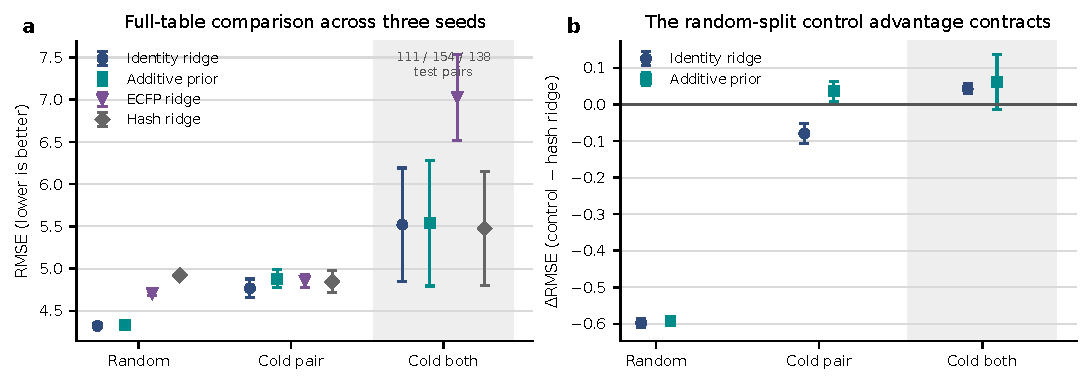
\includegraphics[width=0.96\textwidth]{fig_primary_repeated_entity_result.pdf}
    \caption{Primary full-table result across three seeds. (a) Mean RMSE $\pm$ one standard deviation for identity ridge, additive prior, ECFP ridge, and hash ridge under random, cold-pair, and cold-both-drugs evaluation. The shaded cold-both-drugs region reports the per-seed number of retained unordered test pairs. (b) Paired identity and additive RMSE differences relative to hash ridge, shown as mean $\pm$ one standard deviation across seeds; negative values favor the train-only control. The random-split control advantage contracts after exact-pair reuse is removed and becomes unresolved for the two-new-drug test graphs.}
    \label{fig:primary-result}
\end{figure*}

\subsection{Removing reuse changes the conclusion}

Full-table cold-pair splitting removes exact pair reuse but retains all drugs and cells. Identity ridge reaches RMSE $4.766\pm0.111$, compared with $4.846\pm0.132$ for hash ridge, $4.857\pm0.080$ for ECFP ridge, and $4.882\pm0.105$ for additive prior. The identity--hash gap contracts from 0.597 to 0.080 RMSE, while the identity--ECFP gap contracts from 0.385 to 0.091. Exact-pair reuse is therefore associated with a substantial share of the identity control's random-split advantage over both feature baselines.

Cold-both-drugs changes both the model interpretation and the split stability. Identity ridge reaches $5.520\pm0.671$, additive prior $5.538\pm0.743$, hash ridge $5.477\pm0.675$, and ECFP ridge $7.028\pm0.507$. The large standard deviations for the first three models coincide with test sets ranging from 5,449 to 8,624 rows and 111 to 154 unordered pairs (Table~\ref{tab:split-sizes}). Under this split, identity ridge reduces to an intercept-plus-cell-identity fallback, while additive prior reduces primarily to its cell component. Their available-component cPCS values are near one, but the fixed-denominator values are approximately 0.331 because only the cell component varies. Neither value implies continued access to held-out drug identities, and the small retained graphs make model rankings less stable.

On the common 30k suite, cold-at-least-one-drug brings identity, additive, and hash ridge to RMSE 4.956--4.980, whereas the compact MLPs reach approximately 5.20 and ECFP ridge reaches $5.413\pm0.335$. The SMILES-hash cluster stress favors hash ridge (4.878) over identity (4.953), while additive prior is close (4.897); nearest-training-drug hash cosine remains 0.625--0.667 on average. Cold-cell removes all cell overlap while retaining familiar drugs and pairs. Identity ridge obtains RMSE $4.900\pm0.490$, additive prior $4.952\pm0.502$, ECFP ridge $5.021\pm0.486$, hash ridge $5.175\pm0.470$, descriptor MLP $5.108\pm0.425$, and dual-view MLP $5.272\pm0.559$. The remaining identity advantage is consistent with the retained drug and exact-pair interpolation channels. The corresponding identity and additive $\mathrm{cPCS}^{(3)}$ values remain 0.559 and 0.560.

\begin{figure*}[!t]
    \centering
    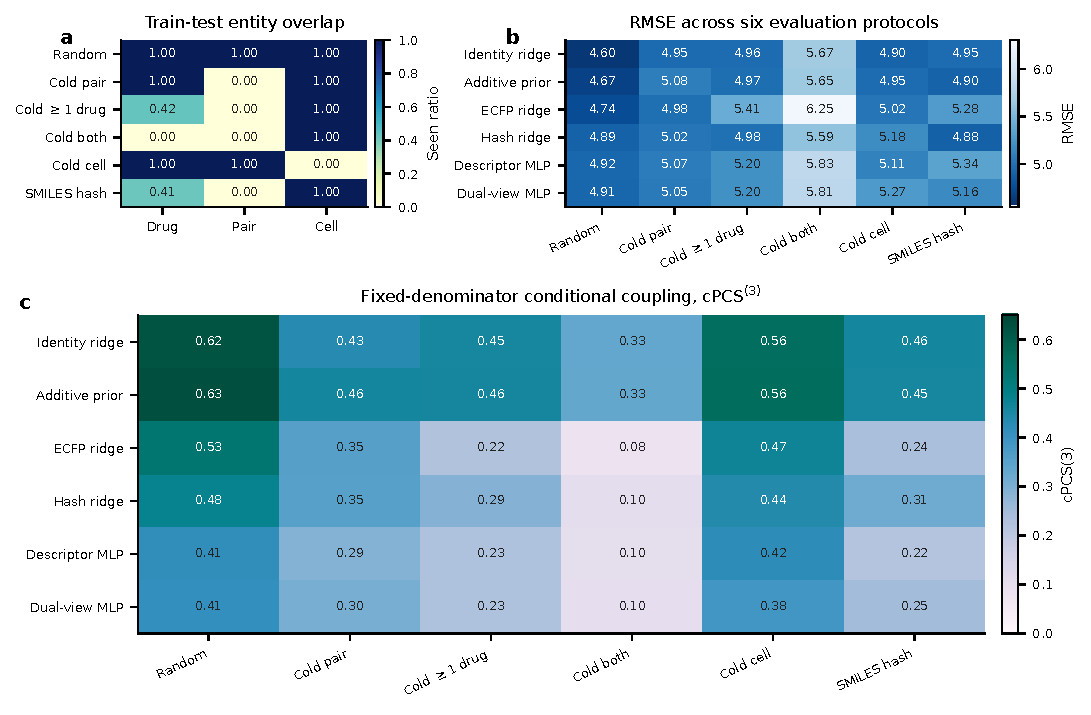
\includegraphics[width=0.96\textwidth]{fig_six_split_audit.pdf}
    \caption{Six evaluation protocols. (a) Mean full-table train--test reuse across three seeds. Drug seen ratio counts test drug slots whose identifier occurs in training; pair and cell seen ratios count test rows whose unordered pair or cell occurs in training. Values are rounded to two decimals, and the random-split pair ratio exceeds 99.99\%. (b,c) Mean RMSE and fixed-denominator $\mathrm{cPCS}^{(3)}$ for six controlled models on the common 30k suite. Unavailable prior components contribute zero, preserving a common denominator. Full-table cold-drug retained and discarded row counts are reported in Table~\ref{tab:split-sizes}.}
    \label{fig:six-split}
\end{figure*}

Figure~\ref{fig:six-split} places random evaluation and five split stresses in one comparison. Random splitting maximizes overlap and favors identity/prior controls; cold-at-least-one-drug and SMILES-hash cluster splits partially remove drug reuse; cold-pair and cold-cell isolate different entity axes; and cold-both-drugs removes both drug and exact-pair reuse while retaining a much smaller, seed-dependent test graph. Each protocol therefore yields a model ordering tied to its transfer regime.

\begin{table}[!t]
\centering
\scriptsize
\setlength{\tabcolsep}{3pt}
\caption{30k multi-seed RMSE (mean $\pm$ SD) on added transfer splits.}
\label{tab:cold}
\begin{tabular}{lccc}
\toprule
Model & Cold-$\geq$1-drug & Cold-both-drugs & SMILES-hash \\
\midrule
Identity ridge & $4.956\pm.370$ & $5.668\pm.298$ & $4.953\pm.229$ \\
Additive prior & $4.972\pm.393$ & $5.649\pm.330$ & $4.897\pm.253$ \\
Hash ridge & $4.980\pm.307$ & $5.593\pm.236$ & $4.878\pm.126$ \\
ECFP ridge & $5.413\pm.335$ & $6.251\pm.380$ & $5.282\pm.294$ \\
Descriptor MLP & $5.202\pm.283$ & $5.826\pm.202$ & $5.339\pm.291$ \\
Dual-view MLP & $5.205\pm.258$ & $5.812\pm.245$ & $5.160\pm.231$ \\
\bottomrule
\end{tabular}
\end{table}

\subsection{External NCI-ALMANAC check}

The separately processed NCI-ALMANAC table contains 306,365 rows, 104 drugs, 5,233 unordered pairs, and 59 cells. All test drugs, pairs, and cells are seen in training under each random split. Pair prior reaches RMSE $53.10\pm0.54$, close to additive prior at $52.70\pm0.48$ and symmetric identity ridge at $52.40\pm0.53$ (Table~\ref{tab:nci}); identity obtains Pearson $0.606\pm0.015$ and PCS $0.566\pm0.001$. This result confirms that strong train-only entity controls also occur in a second high-reuse random-split table. Because the CellMiner scores use a different definition and scale and the processed table lacks the harmonized feature representation used for DrugComb, this check does not establish the same feature-model ranking across datasets.

\begin{table}[!t]
\centering
\scriptsize
\caption{Three-seed NCI-ALMANAC random-split test results (mean $\pm$ SD).}
\label{tab:nci}
\resizebox{\columnwidth}{!}{%
\begin{tabular}{lrrr}
\toprule
Model & RMSE & Pearson & PCS \\
\midrule
Global mean & $65.68\pm1.42$ & -- & -- \\
Drug prior & $63.72\pm1.39$ & $.282\pm.003$ & $.486\pm.002$ \\
Pair prior & $53.10\pm.54$ & $.595\pm.016$ & $.486\pm.003$ \\
Cell prior & $65.23\pm1.41$ & $.116\pm.002$ & $.336\pm.002$ \\
Additive prior & $52.70\pm.48$ & $.597\pm.014$ & $.590\pm.001$ \\
Identity ridge & $52.40\pm.53$ & $.606\pm.015$ & $.566\pm.001$ \\
\bottomrule
\end{tabular}
}
\end{table}

\subsection{Supporting check: the split conclusion persists across labels}

The label check compares split-level degradation for ZIP, Bliss, Loewe, and HSA on their respective scales (Fig.~\ref{fig:support}c). Relative to its random-split RMSE, the symmetric identity control worsens by 10.6--23.3\% under cold-pair, 14.9--21.6\% under cold-at-least-one-drug, and 1.6--8.7\% under cold-cell evaluation. Every label therefore shows a positive random-to-cold RMSE increase.

\section{Supporting Diagnostics}

\subsection{Supporting check: adjusted coupling behaves as intended}

All three synthetic cases have RMSE 1.0 by construction (Fig.~\ref{fig:supporting-diagnostics}b). Adjusted diagnostics are near zero for label-only and nonlinear label--prior association. Direct residual-prior use is separated by cPCS 0.649, incremental $R^2$ 0.106, and null excess 0.190, matching the intended diagnostic behavior.

\subsection{Supporting check: CPB tracks feature-removal tradeoffs}

Within the cold-pair RMSE range shared by learned, shuffled, and random controls, random-cluster settings attain the lowest cPCS at matched error (Fig.~\ref{fig:supporting-diagnostics}a). On the full table, learned CPB reaches RMSE $5.248\pm0.090$ and cPCS $0.336\pm0.090$, while random-cluster CPB reaches RMSE $5.197\pm0.081$ and cPCS $0.331\pm0.036$. CPB therefore provides a controllable feature-removal sweep. The matched controls make the observed tradeoff more consistent with generic information removal than with a unique contribution from learned prototype geometry.

\begin{figure*}[!t]
    \centering
    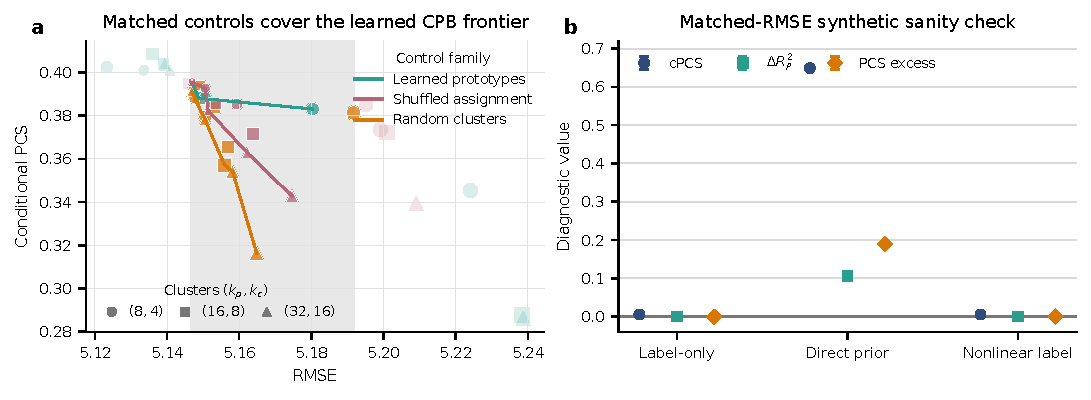
\includegraphics[width=0.96\textwidth]{fig_supporting_coupling_checks.pdf}
    \caption{Supporting diagnostics. (a) Cold-pair CPB sweeps over $(k_p,k_c)\in\{(8,4),(16,8),(32,16)\}$ and $\lambda\in\{0,0.25,0.50,0.75,1.00\}$. Line color denotes the control family; circles, squares, and triangles denote the three cluster grids, and marker size increases with $\lambda$. Each point averages seeds 0, 42, and 123. Lines trace each control family's Pareto frontier. The shaded interval is the RMSE range shared by learned, shuffled-assignment, and random-cluster controls. (b) Matched-RMSE synthetic sanity check over 20 seeds. Adjusted coupling remains near zero for label-only and nonlinear label--prior cases and becomes positive when prediction directly includes prior residuals.}
    \label{fig:supporting-diagnostics}
\end{figure*}

\subsection{The primary audit remains lightweight at full scale}

On all 287,268 rows, identity and additive controls finish in 0.60 and 0.38 seconds. Hash ridge takes 92.40 seconds with a 4.64 GB peak working set; learned residual CPB takes 38.18 seconds with 1.89 GB. The same qualitative resource trend appears at 25k, 50k, and 100k (Fig.~\ref{fig:support}b). The complete audit therefore runs comfortably on a 16 GB workstation before expensive architecture search.

\begin{figure*}[!t]
    \centering
    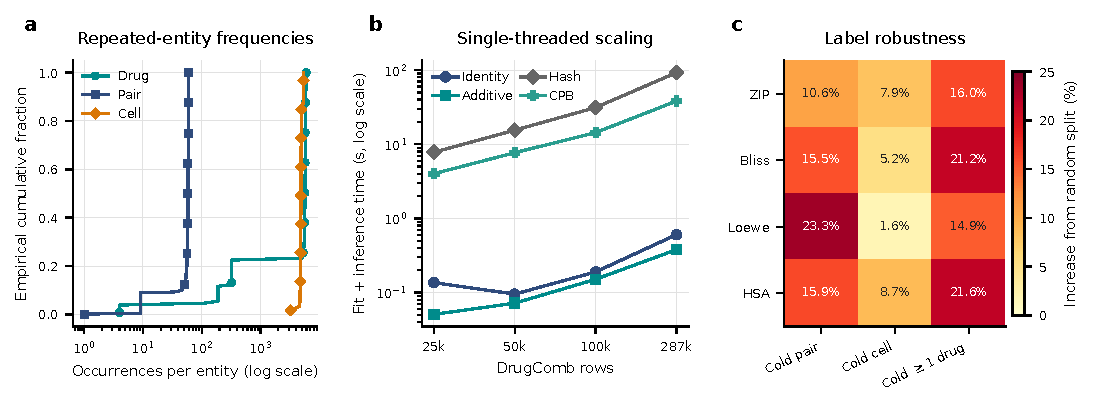
\includegraphics[width=0.96\textwidth]{fig_scaling_frequency_label_support.pdf}
    \caption{Supporting data-centric checks. (a) Full-table empirical cumulative distributions: drug occurrence counts both drug slots, whereas unordered-pair and cell occurrence count rows. (b) Single-threaded fit-plus-inference time from 25k rows to the complete 287,268-row table. (c) Full-table seed-42 identity-control RMSE increase from random to cold splits for ZIP, Bliss, Loewe, and HSA, expressed relative to each label's random-split RMSE.}
    \label{fig:support}
\end{figure*}

\section{Discussion}

The primary finding is that random row splitting substantially rewards repeated-entity interpolation. The benchmark contains hundreds of thousands of rows, yet its test rows are constructed from a small set of drugs, pairs, and cells that are almost entirely familiar from training. In that maximal-reuse regime, identity ridge improves on ECFP and hash ridge by 0.385 and 0.597 RMSE, respectively, while additive prior performs almost identically to identity ridge. Removing exact-pair reuse contracts those gaps to 0.091 and 0.080 RMSE. Requiring at least one new drug makes identity, additive, and hash ridge comparable on the common 30k suite, and the SMILES-hash cluster stress favors hash ridge. These observed contractions identify familiar-entity interpolation as a major component of the random-split advantage within the evaluated baseline family.

Different cold splits answer different deployment questions. Cold-pair tests new combinations of familiar drugs and cells. Cold-at-least-one-drug tests partial drug novelty. Cold-both-drugs removes both drug and exact-pair reuse, retains cell information, and produces a much smaller, seed-dependent graph. Cold-cell removes cell identity while leaving drugs and pairs familiar, a setting in which identity controls remain competitive. Reporting the intended transfer regime therefore gives each leaderboard a concrete deployment meaning.

The NCI-ALMANAC check strengthens the data-centric conclusion at the level supported by its available fields. Strong pair, additive, and identity baselines appear on a separately processed large table with complete random-split entity reuse and a different score scale. This establishes that strong entity-only random-split predictability is not unique to the processed DrugComb table, while leaving cross-dataset feature-model rankings open. In Big Data benchmarks, row count alone can overstate evaluation diversity when the repeated-entity graph contains extensive train--test reuse.

Conditional PCS, incremental prior $R^2$, and the moment-matched heuristic null reveal prediction--prior dependence beyond simple linear label alignment. The synthetic cases verify the expected response to direct residual-prior use. The CPB sweep further shows that learned, shuffled, and random removals occupy a shared error--coupling frontier. This pattern links the tradeoff primarily to information removal. Together, these diagnostics explain how the main repeated-entity effect appears in model outputs and residual feature spaces.

The practical recommendation is inexpensive: report global, prior-only, and identity baselines; publish entity-frequency and train--test overlap audits; include deployment-matched cold splits; disclose retained and discarded graph sizes; and use grouped uncertainty estimates. These checks can run before costly architecture searches and reveal how much of a benchmark improvement comes from familiar-entity interpolation and how much persists in the intended transfer setting.

\section{Limitations}

The evaluated model suite contains identity and prior controls, a standard Morgan-fingerprint ridge, a character-hash ridge, and descriptor and dual-view MLPs built from the common TDC fields. Architecture-specific replication of DeepSynergy, MatchMaker, DeepDDS, TranSynergy, and MARSY would require their genomic, perturbational, target, and graph inputs. The reported model rankings therefore apply to the controlled baseline family and split protocols evaluated here.

The representation-cluster split uses unsupervised character SMILES hashes and SVD over all unique drugs, while future work can add scaffold and similarity-constrained partitions. Cold-both-drugs retains cell priors and discards cross-group pairs, producing seed-dependent test graphs. CPB controls match mean removed centroid energy; richer controls could additionally match directional information loss. Three split seeds and 100 bootstrap replicates balance grouped uncertainty estimation with workstation-scale computation. Source, study, assay, dose-grid, and batch columns would enable further source-aware audits. NCI-ALMANAC supplies a random-split entity-control check on its native score scale; harmonized molecular and cell features would be required for a matched cross-dataset model comparison.

\section{Conclusion}

Random row splitting in the evaluated drug synergy benchmarks substantially rewards repeated-entity interpolation. Under maximal reuse, train-only identity and prior controls match or outperform the evaluated Morgan-fingerprint, hash-feature, and compact neural baselines; after exact-pair or drug reuse is removed, their advantage contracts, disappears, or becomes dependent on the remaining entity channel and retained test graph. NCI-ALMANAC also exhibits strong random-split train-only controls under complete entity reuse. Our lightweight audit connects entity overlap, simple train-only controls, random evaluation, and five transfer stresses in one workflow. Reliable synergy evaluation should report what entities repeat, which transfer regime is tested, how simple train-only controls perform, and how conclusions change when reuse channels are removed.

\medskip
\noindent\textbf{Funding.}
This research was funded by the National Science and Technology Council, Taiwan (grant number NSTC115-2221-E-038-012-MY3).

\medskip
\noindent\textbf{Data and Code Availability.}
The datasets used in this study were obtained from publicly available sources. The preprocessing scripts, dataset split definitions, model configurations, aggregated results, and evaluation code are publicly available at \url{https://github.com/WenYuxin2003/repeated-entity-audit-drug-synergy}.

\balance
\begin{thebibliography}{99}

\bibitem{drugcomb2019}
B. Zagidullin \emph{et al.}, ``DrugComb: an integrative cancer drug combination data portal,'' \emph{Nucleic Acids Research}, vol. 47, no. W1, pp. W43--W51, 2019, doi: 10.1093/nar/gkz337.

\bibitem{drugcombdb2020}
H. Liu, W. Zhang, B. Zou, J. Wang, Y. Deng, and L. Deng, ``DrugCombDB: a comprehensive database of drug combinations toward the discovery of combinatorial therapy,'' \emph{Nucleic Acids Research}, vol. 48, no. D1, pp. D871--D881, 2020, doi: 10.1093/nar/gkz1007.

\bibitem{nci2019almanac}
D. A. Close, A. X. Wang, S. J. Kochanek, T. Shun, J. L. Eiseman, and P. A. Johnston, ``Implementation of the NCI-60 human tumor cell line panel to screen 2260 cancer drug combinations,'' \emph{SLAS Discovery}, vol. 24, no. 3, pp. 242--263, 2019.

\bibitem{deepsynergy2018}
K. Preuer, R. P. I. Lewis, S. Hochreiter, A. Bender, K. C. Bulusu, and G. Klambauer, ``DeepSynergy: predicting anti-cancer drug synergy with deep learning,'' \emph{Bioinformatics}, vol. 34, no. 9, pp. 1538--1546, 2018, doi: 10.1093/bioinformatics/btx806.

\bibitem{matchmaker2022}
H. I. Kuru, O. Tastan, and A. E. Cicek, ``MatchMaker: a deep learning framework for drug synergy prediction,'' \emph{IEEE/ACM Trans. Comput. Biol. Bioinf.}, vol. 19, no. 4, pp. 2334--2344, 2022, doi: 10.1109/TCBB.2021.3086702.

\bibitem{deepdds2022}
J. Wang, X. Liu, S. Shen, L. Deng, and H. Liu, ``DeepDDS: deep graph neural network with attention mechanism to predict synergistic drug combinations,'' \emph{Briefings in Bioinformatics}, vol. 23, no. 1, bbab390, 2022, doi: 10.1093/bib/bbab390.

\bibitem{transynergy2021}
L. Liu \emph{et al.}, ``TranSynergy: mechanism-driven interpretable deep neural network for the synergistic prediction and pathway deconvolution of drug combinations,'' \emph{PLOS Computational Biology}, vol. 17, no. 2, e1008653, 2021.

\bibitem{marsy2023}
M. R. El Khili, S. A. Memon, and A. Emad, ``MARSY: a multitask deep-learning framework for prediction of drug combination synergy scores,'' \emph{Bioinformatics}, vol. 39, no. 4, btad177, 2023, doi: 10.1093/bioinformatics/btad177.

\bibitem{geirhos2020shortcut}
R. Geirhos \emph{et al.}, ``Shortcut learning in deep neural networks,'' \emph{Nature Machine Intelligence}, vol. 2, pp. 665--673, 2020.

\bibitem{brown2023shortcut}
A. Brown \emph{et al.}, ``Detecting shortcut learning for fair medical AI using shortcut testing,'' \emph{Nature Communications}, vol. 14, art. 4314, 2023, doi: 10.1038/s41467-023-39902-7.

\bibitem{dewulf2021cold}
P. Dewulf, M. Stock, and B. De Baets, ``Cold-start problems in data-driven prediction of drug--drug interaction effects,'' \emph{Pharmaceuticals}, vol. 14, no. 5, art. 429, 2021, doi: 10.3390/ph14050429.

\bibitem{datasail2025}
R. Joeres, D. B. Blumenthal, and O. V. Kalinina, ``Data splitting to avoid information leakage with DataSAIL,'' \emph{Nature Communications}, vol. 16, art. 3337, 2025, doi: 10.1038/s41467-025-58606-8.

\bibitem{synverse2025}
N. Tasnina, M. Haghani, and T. M. Murali, ``SynVerse: a modular framework for building and evaluating deep learning-based drug synergy prediction models,'' \emph{Briefings in Bioinformatics}, vol. 26, no. 6, bbaf676, 2025, doi: 10.1093/bib/bbaf676.

\bibitem{graphsynergy2021}
J. Yang, Z. Xu, W. K. K. Wu, Q. Chu, and Q. Zhang, ``GraphSynergy: a network-inspired deep learning model for anticancer drug combination prediction,'' \emph{J. Am. Med. Inform. Assoc.}, vol. 28, no. 11, pp. 2336--2345, 2021, doi: 10.1093/jamia/ocab162.

\bibitem{prodeepsyn2022}
X. Wang \emph{et al.}, ``PRODeepSyn: predicting anticancer synergistic drug combinations by embedding cell lines with protein--protein interaction network,'' \emph{Briefings in Bioinformatics}, vol. 23, no. 2, bbab587, 2022, doi: 10.1093/bib/bbab587.

\bibitem{mmsyn2024}
Y. Pang, Y. Chen, M. Lin, Y. Zhang, J. Zhang, and L. Wang, ``MMSyn: a new multimodal deep learning framework for enhanced prediction of synergistic drug combinations,'' \emph{J. Chem. Inf. Model.}, vol. 64, no. 9, pp. 3689--3705, 2024, doi: 10.1021/acs.jcim.4c00165.

\bibitem{chemicalx2022}
B. Rozemberczki \emph{et al.}, ``ChemicalX: a deep learning library for drug pair scoring,'' in \emph{Proc. 28th ACM SIGKDD Conf. Knowledge Discovery and Data Mining}, 2022, pp. 3819--3828, doi: 10.1145/3534678.3539023.

\bibitem{networkprop2018}
H. Li, T. Li, D. Quang, and Y. Guan, ``Network propagation predicts drug synergy in cancers,'' \emph{Cancer Research}, vol. 78, no. 18, pp. 5446--5457, 2018, doi: 10.1158/0008-5472.CAN-18-0740.

\bibitem{amzallag2019}
A. Amzallag, S. Ramaswamy, and C. H. Benes, ``Statistical assessment and visualization of synergies for large-scale sparse drug combination datasets,'' \emph{BMC Bioinformatics}, vol. 20, art. 83, 2019.

\bibitem{musyc2021}
C. T. Meyer \emph{et al.}, ``MuSyC is a consensus framework that unifies multi-drug synergy metrics for combinatorial drug discovery,'' \emph{Nature Communications}, vol. 12, art. 4607, 2021, doi: 10.1038/s41467-021-24789-z.

\bibitem{bansal2014}
M. Bansal \emph{et al.}, ``A community computational challenge to predict the activity of pairs of compounds,'' \emph{Nature Biotechnology}, vol. 32, pp. 1213--1222, 2014.

\bibitem{tdc2021}
K. Huang \emph{et al.}, ``Therapeutics Data Commons: machine learning datasets and tasks for therapeutics,'' in \emph{Proc. NeurIPS Datasets and Benchmarks}, 2021.

\bibitem{lin2025tapb}
G. Lin \emph{et al.}, ``TAPB: an interventional debiasing framework for alleviating target prior bias in drug-target interaction prediction,'' \emph{Nature Communications}, vol. 16, art. 10867, 2025, doi: 10.1038/s41467-025-66915-1.

\bibitem{rogers2010ecfp}
D. Rogers and M. Hahn, ``Extended-connectivity fingerprints,'' \emph{J. Chem. Inf. Model.}, vol. 50, no. 5, pp. 742--754, 2010, doi: 10.1021/ci100050t.

\bibitem{sklearn2011}
F. Pedregosa \emph{et al.}, ``Scikit-learn: machine learning in Python,'' \emph{Journal of Machine Learning Research}, vol. 12, pp. 2825--2830, 2011.

\end{thebibliography}

\end{document}
